% Chapter 5

\chapter{\textsf{Painless} integration with ProActive} 
\label{chap:extraction} 


\epigraph{\textit{“Many will call me an adventurer - and that I am, only one of a different sort: 
                             one of those who risks his skin to prove his platitudes."}}{Che Guevara}



\minitoc

\lhead{Chapter 5. \emph{\textsf{Painless} integration with ProActive}} % This is for the header on each page - perhaps a shortened title


	This Chapter proposes a new \ac{ADL}, named \textsc{Painless}, and discusses its associated tool support.
	Section \ref{sec:painlessapproach} describes the undertaken approach for providing an
	extension to the ProActive middleware supporting the interpretation of 
	\textsc{Painless} specifications.
	The syntax and semantics of \textsc{Painless} are presented in Section \ref{sec:painless}. Specification
	examples are also explained. Finally, Section \ref{sec:painlessdiscussion} concludes this Chapter.

	Our GCM/ProActive extension implementation	 is freely available online, and contains
	the examples discussed in this Chapter and several others. The interested reader 
	is pointed to website\footnote{The \textsc{Painless} extension for the ProActive middleware
	is available online at: \url{http://www-sop.inria.fr/members/Nuno.Gaspar/Painless.php}} 
	of its development for more details.


%----------------------------------------------------------------------------------------


\section{Integration approach}
\label{sec:painlessapproach}

	
		Typically, one uses an \ac{ADL} as a means to specify the 
	software architecture. This promotes separation of concerns
	and compels the software architect to accurately define structural requisites. Nevertheless,
	this task is seldom trivial as arbitrarily complex architectures may need to be defined.
	It is thus important to provide the means for expressive and intuitive, yet reliable, specifications.	
	As discussed in Section \ref{sec:proactive}, the ProActive middleware supports the specification
	of \ac{GCM} architectures by means of its own \ac{ADL} --- for instance, Listing \ref{lst:starteradl}
	exemplified one such architecture specification.
				
	 However, the \ac{GCM} \ac{ADL} lacks support for architectural
	reconfigurations and parametrization. Further, it is XML-based: while it may be suitable
	for tools, it is a rather verbose and static description of the architecture.
		
	To this end, \textsc{Painless} supports both the definition
	of parametrized architectures and the specification of reconfigurations in a declarative style. This,
	facilitates deployment tasks and gives a more comprehensive understanding
	of the application's topology.  

	In the following we detail our approach for extending the ProActive middleware
	with the capacity to cope \textsc{Painless} specifications. In particular, we show how 
	we leverage \textsc{Mefresa}'s apparatus to provide an automated means to reduce
	\textsf{operations}, and how this is subsequently used as a back-end for evaluating \textsf{Painless}
	specification's compliance w.r.t. the \ac{GCM} requirements.
	

\subsection{Computing \textsf{states} from \textsf{operations}}
\label{sub:buildstate}


	As seen in Section \ref{sec:op}, one can check the feasibility
	of reducing an \textsf{operation} by interactively applying	
	its reduction rules (see Table \ref{tab:semantics}) and attempting to prove the required premises.
	This ability is of great value when attempting to prove arbitrary complex
	properties about potentially parametrized architectures. Indeed, proof
	assistants are notoriously known for their strength in performing 
	inductive proofs.

	Yet, if the intention is to build a \textsf{state} representing
	the result of an \textsf{operation} reduction, then we would be better
	with a function performing such task. This is the purpose of the
	function depicted by Listing \ref{lst:buildstate}.
	
	
			\lstinputlisting[language=Coq, stepnumber=1, 
	                      caption={Excerpt of the \textsf{build\_state} function definition}, 
	                      %firstnumber=19,
	                      label=lst:buildstate]{listings/chapter5/buildstate.tex}				
	
	
	\noindent The above excerpt shows how we can use a function to compute the result
	of an arbitrary \textsf{operation} reduction. Basically, it pattern matches on the parameter \textsf{op} (line 2),
	proceeds depending on the matched constructor. For instance, if it is a \textsf{MK\_component},
	it performs the adequate checks w.r.t. to the \textsf{SMakeComponent} proof rule, 
	and invokes the \textsf{add\_component} function (lines 3-9). As expected,
	\textsf{valid\_component\_path\_bool} is a boolean function checking
	if path \textsf{p} points to an existing \textsf{component} in the \textsf{state} \textsf{init}.
	\textsf{no\_id\_clash} checks that the identifier \textsf{i} is not already
	used by another \textsf{component} at the same hierarchical level. For last,
	\textsf{dec\_component} computes whether the \textsf{component} to be
	added is well-formed.	
	
	Apart from the
	\textsf{Seq} and \textsf{Done} constructors, the remaining \textsf{operation} 
	 constructors are handled analogously. \textsf{Seq} is composed by two \textsf{operations} (line 13),
	 the leftmost \textsf{operation} is fully reduced, and the resulting \textsf{state} is used
	 for reducing the rightmost \textsf{operation} (lines 14-18). \textsf{Done} means that the end of 
	 the \textsf{operation} was reached, and it simply returns the current \textsf{state}.
	 
	 
	 	Another important note regards the use of the \textsf{option} type as return type of this
	 function. This is due to the fact that it only returns a \textsf{state} if it was able to \textsf{reduce}
	 the given \textsf{operation}, otherwise it simply returns \textsf{None}.
	This should come as no surprise, as it is not always the case that an \textsf{operation}
	can be fully reduced. Further, as discussed in Chapter \ref{chap:mefresa},
	the \textsf{validty} theorem (see Listing \ref{lst:validity}) enunciates that reducing
	an \textsf{operation} to \textsf{Done} from a well-formed \textsf{state} yields a 
	well-formed \textsf{state}.	
	Naturally, the analogous behaviour is expected from the \textsf{build\_state} function. 	
	Further, we also expect it to  always be able  to compute a resulting \textsf{state} from an
	\textsf{operation op}, whenever it is possible to reduce \textsf{op} to \textsf{Done}.	
	In short, we want the computational counterpart of the
	reflexive transitive closure of the \textsf{step} predicate. Listing \ref{lst:buildstatecorrect}
	depicts the relevant Theorem.
	

   \lstinputlisting[language=Coq, numbers=left, label=lst:buildstatecorrect, caption=\textsf{validity} statement]
                          {listings/chapter5/buildstatecorrect.tex}			


	\noindent Proving \textsf{buid\_state\_correctness} requires a case analysis on the \textsf{operation}
	constructors, and relating the boolean checks made in \textsf{build\_state}	
	with the premises of  the \textsf{step} predicate.	
	
		By the above Theorem we know that \textsf{build\_state} is both 
	\textit{complete} and \textit{sound}. Complete since 
	starting from a \textsf{well formed} 
	state \textsf{s}, it always computes a state \textsf{s'} holding the effects of \textsf{op} 
	whenever \textsf{op} can be proved to be reduced to \textsf{Done} attaining \textsf{s'}.
	Sound, as we can always prove that
	\textsf{op}  can be reduced to \textsf{Done} and attain a state \textsf{s'} provided that
	 \textsf{build\_state} applied to \textsf{op} and \textsf{s} returns \textsf{s'}.
%%%

	%From Lemma \ref{th:wfempty} we know that an empty \textsf{state} is well-formed. 
	Considering the context of a component-based application
	life-cycle, one deploys its application by performing an operation $op$ on an
	empty \textsf{state}, and thus well-formed (by Lemma \ref{th:wfempty}). Then, if $op$ can indeed
	be reduced, we reach a well-formed \textsf{state s} (by Theorem \ref{lst:validity}). 
		
	%%%

	Performing an architectural reconfiguration boils 
	down to applying an \textsf{operation} $op$' to \textsf{s}, leading to yet another
	well-formed \textsf{state s'} --- provided that $op$' can indeed be reduced ---, and
	this cycle can be repeated indefinitely. Indeed, there is no need to explicitly compute the 
	well-formedness of the attained \textsf{states}, as it is provably guaranteed. 
	There is however such a need regarding their well-typedness.
	%This is the purpose of the $well\_typed\_bool : component \rightarrow boolean$ function.
		
	 Basically, we end up with all the necessary tools to compute whether a given \textsf{operation},
	 of deployment or reconfiguration nature, can be safely applied.  The function
	 \textsf{build\_state} (see Listing \ref{lst:buildstate}) constructs the resulting (provably well-formed) 
	 \textsf{state} from an \textsf{operation}, and \textsf{well\_typed\_bool} (see Listing \ref{lst:wtbool})
	 checks whether a given \textsf{state} is well-typed.	
	 
	 
\subsection{Certified code, \textsc{Painless} interpreter, and the ProActive middleware}
\label{sub:painlessproactive}

 
	As discussed above, the functions  \textsf{build\_state} and \textsf{well\_typed\_bool}
	compute the resulting \textsf{state} from a given \textsf{operation}, and
	check for a \textsf{state}'s well-typedness, respectively. This is of great value, yet,
	it falls short w.r.t. informing a user about a cause of failure. For instance, an
	\textsf{operation} may not be able to be reduced since it attempts to remove
	a \textsf{component} that is still connected to another. For such cases, it 
	is important to provide some feedback providing insight on the root of the issue.
		 
		 
	We define custom versions of the involved functions. For instance,	 
	the function \textsf{custom\_build\_state :operation $\rightarrow$ state $\rightarrow$ (option state * option wf\_error\_msg)},
	behaves as \textsf{build\_state}, but carries back a \textsf{wf\_error\_msg} value in case of an issue.	 
	Listing \ref{lst:errormsg} depicts the definition of the \textsf{wf\_error\_msg} datatype. 				
	 				
      \lstinputlisting[language=Coq, numbers=left, label=lst:errormsg, caption=\textsf{wf_error_msg} type definition]
                          {listings/chapter5/errormsg.tex}			 				
                          
                          
	\noindent Basically, it defines a constructor for each \textsf{operation} constructor whose reduction
	actually produces an effect to the current \textsf{state} (liens 7-11). Further, their elements hold all the
	relevant information for adequately identifying the origin of an issue in an \textsf{operation} reduction.        
    For instance, the \textsf{ErrorMkComponent} (line 7) holds the identifier, \textsf{path}, 
    and \textsf{wf\_error} value of the involved \textsf{component}.          
                          
	For the sake of clarity, Listing \ref{lst:custombuildstate} depicts an excerpt of the
	\textsf{custom\_build\_state} illustrating how error-reporting is handled.                          
                          
                          
        \lstinputlisting[language=Coq, numbers=left, label=lst:custombuildstate, caption=\textsf{custom_build_state} function definition]
                          {listings/chapter5/custombuildstate.tex}			                   
                    
                    
	\noindent Indeed, it is a rather simple approach: at each boolean check, it returns its 
	associated cause if a \textit{false} value is obtained  (lines 6, 9, 12).                    
                    
                    
     While this error-reporting approach is simple enough, it is important to ensure that it causes no
     conflict with the behaviour of the original \textsf{build\_state} function. Moreover, we also expect it
     to be able to always report back an error message whenever it is not possible to
     reduce an \textsf{operation}. This addressed by Lemma \textsf{custom\_build\_state\_correct} 
     as depicted by Listing \ref{lst:custombuildstatecorrect}.                
                          
	 				
	\lstinputlisting[language=Coq, numbers=left, label=lst:custombuildstatecorrect, caption=\textsf{custom\_build\_state\_correct} lemma]
                      {listings/chapter5/custombuildstatecorrect.tex}			 				
	 				
	\noindent The above lemma is proved by case analysis of the \textsf{operation} datatype.
	It poses no particular challenge, as indeed both functions have a similar structure.	
	
	As expected, an analogous approach is used regarding the \textsf{well\_typed\_bool} function,
	that is, we have a function \textsf{custom_well_typed_bool : state $\rightarrow$ option wt_error_msg},
	reporting back the cause of a well-typedness non-compliance.
	

	As discussed in Subsection \ref{sub:coqextract}, Coq is able to extract functional code
	into OCaml. We use this feature to extract both \textsf{custom\_build\_state} and 
	\textsf{custom\_well\_typed\_bool}. Then, through \textit{OCaml-Java} \cite{conf/sfp/Clerc12}, 
	we obtain a Java library implementing these two functions. 
	
	Figure \ref{fig:integration} depicts the overall approach for providing an
	extension to the ProActive middleware coping with \textsc{Painless} specifications.
						
					
	\begin{figure}[H]
	\centering
	 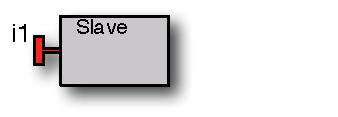
\includegraphics[scale=1]{figures/chapter5/starter.pdf} 	
   	\caption{Simple GCM application example}
   	\label{fig:integration}
	\end{figure}
	
	
	\noindent The \textsc{Painless} interpreter is directly written in OCaml, and also
	compiled to Java bytecode with OCaml-Java. 	
	Basically, its only task is to interpret a \textsc{Painless} expression to 
	\textsc{Mefresa}'s \textsf{operation} language. This is the case for both
	deployment and reconfiguration expressions.	
	Then, the resulting
	\textsf{operation} is reduced with \textsf{custom\_build\_state}. If
	no issue is reported back, then the returned \textsf{state} is checked
	with \textsf{custom\_well\_typed\_bool}. Provided that no well-typedness
	issue is detected, the \textsf{operation} is mapped to the adequate methods	
	composing the GCM/ProActive API. Further, the object holding the
	\textsf{state}'s structure is kept for subsequent reconfiguration
	tasks.
		
		It should also be noted that whenever an error is reported back,
	from \textsf{custom\_build\_state} or \textsf{custom\_well\_typed\_bool},
	a Java exception holding all the relevant information is thrown. This
	permits to adequately react without stopping the application. Indeed,
	a GCM/ProActive application requires a component 
	to stop its execution in order to perform
	a structural reconfiguration. In our case, we evaluate
	its compliance with the \ac{GCM} specification before actually
	starting the deployment/reconfiguration.
		
	
\section{The \textsc{Painless} architecture description language}
\label{sec:painless}

	\textsc{Painless} is a \textit{\textbf{p}arametrized \textbf{a}rch\textbf{i}tecture 
	descriptio\textbf{n} \textbf{l}anguag\textbf{e} for \textsf{Mefre\textbf{s}a}}. Basically,
	it provides the software architect with the ability to write parametrized architectures
	and its possible structural reconfigurations in a declarative style. An excerpt of
	its grammar is defined by Table \ref{tab:xyz}.

		%\begin{center}
		\begin{table}[h!]
		\begin{tabular}{ l c l }
		 % \textbf{btype}  & ::= & \ \ \blue{Normal} 	\textbf{exp} \textbf{exp} \textbf{exp} \textbf{exp} \textbf{exp}\\	
          %                        &      & 	\textbar\ \blue{Import} 	\textbf{exp} \textbf{exp} \textbf{exp} \textbf{exp}\\		
           %                       &      & 	\textbar\ \blue{Export} 	\textbf{exp} \textbf{exp} \textbf{exp} \textbf{exp}\\					   
		%						   &      &  \\ 
 		   \textbf{exp}     & ::=   &  \ \ n \textbar\ true \textbar\ false \textbar\ $[ ]$  \textbar\ $str$ \textbar\ x \textbar\ \blue{mk} \textbf{exp}  \textbar\ \blue{rm} \textbf{exp}   \textbar\ \blue{skip} \\
 		                           &        & \textbar\ \blue{Component} \textbf{exp}$_1$ ... \textbf{exp}$_6$ \textbar\ \blue{Interface} \textbf{exp}$_1$ ... \textbf{exp}$_7$ \textbar\ \blue{Binding} \textbf{bexp} \\
			                       &        &  \textbar\ \textbf{exp} :: \textbf{exp}  \textbar\ \textbf{exp} = \textbf{exp}  \textbar\  \textbf{exp} $+$ \textbf{exp}  \textbar\  \textbf{exp} $-$ \textbf{exp} \\  
			                       &        &  \textbar\ \blue{if} \textbf{exp} \blue{then} \textbf{exp} \blue{else} \textbf{exp}  \textbar\  \textbf{exp} \textbf{exp} \textbar\  \textbf{exp} ; \textbf{exp}  \\
			                       &        &  \textbar\ \blue{match} \textbf{exp} \blue{with} \textbf{pat}$_1$ $\rightarrow$ \textbf{exp}$_1$  ...  
			                                                                                                               \textbf{pat}$_k$ $\rightarrow$ \textbf{exp}$_{k \geq 1}$ 
			                                                                                                               \blue{end} \\  
	%		                       &        &  \textbar\ \blue{let} P = \textbf{exp} \blue{in} \textbf{exp} \textbar\ \blue{let rec} P = \textbf{exp} \blue{in} \textbf{exp} \\  		                       
			                       &        &  \\
			 \textbf{decl}   & ::=  &  \blue{let} P = \textbf{exp}  \textbar\ \blue{let rec} P = \textbf{exp}\\        
			                      &         & \\
			   \textbf{rcfg}     & ::=   &  \blue{Reconfiguration} \textit{str} arg$_0$ ... arg$_k$\textbf{:} \textbf{decl}$_0$ ... \textbf{decl}$_k$ \blue{reconfigure} \textbf{exp}  \\
	%           \textbf{rcfg}     & ::=   &  \blue{Reconfiguration} \textit{str} \textbf{:} \textbf{exp}  \\
			                      &        &  \\  
	     \textbf{arch}    &  ::=   & \blue{Architecture} \textit{str} \textbf{:} \textbf{decl}$_0$ ... \textbf{decl} $_{k\geq 0}$ \blue{deploy} \textbf{exp} \textbf{rcfg}$_0$ ... \textbf{rcfg}$_{h \geq 0}$ \\          
	     % \textbf{arch}    &  ::=   & \blue{Architecture} \textit{str} \textbf{:} \textbf{exp} \textbf{rcfg}$_0$ ... \textbf{rcfg}$_{k \geq 0}$ \\  
	\end{tabular}
	\caption{\textsc{Painless} syntax (excerpt)}	
	\label{tab:xyz}
	\vspace{-0.5cm}	
	\end{table}
	%\end{center}
	
	
	
	%The reader with a taste for functional programming will recognize some resemblance 		
	%with the OCaml programming language. Indeed, its expressive yet concise 	
	%trait made it a natural influence. 
		
		
	%VALUES like External/internal, mandatory/optional, etc are also Normal Forms...		
		
		Its elementary --- or \textit{normal forms} --- expressions include natural numbers, 
	booleans, lists, and strings.	Naturally, one can also use variables. Making and removing
	elements from the component architecture is achieved by the polymorphic 
	\textsf{mk} and \textsf{rm}, respectively. As expected, \textsf{skip} is idempotent. 
	Components, interfaces and bindings are also first-class citizens --- where \textsf{bexp}
	is an expression for the three types of bindings. 
	 Facilities for manipulating lists, comparison, and
	binary operators such as \textsf{+} and \textsf{-} are also built-in features.
	The standard \textsf{if-then-else}, function call, sequence \textbf{;} and \textsf{match} 
	constructors	 conclude	the range of allowed expressions. \textbf{decl} acts as a
	declaration layer composed by the usual (potentially recursive) \textsf{let} definitions,
	indexed by a parameter \textit{P}.	
		
			
		Therefore, an architecture \textbf{arch} is composed by a string \textsf{str} representing its name,
		$k\geq 0$ declarations, and an expression describing the application deployment topology. Further, it may contain 
	$h \geq 0$ similarly defined reconfigurations.
				
		
	%	Indeed, \textsc{Painless} offers the basic	 features of a functional programming language. Recursion,
	%pattern-matching and side-effect free are among its main characteristics. This provides a rather
	%simple and intuitive way to express architectures. %For instance, an elementary ingredient is
	%the creation of primitive components. These do not possess subcomponents and bindings. One 
	%can easily devise a function as a shorthand for primitive components as depicted by
	%Listing \ref{lst:c}.
		
	%\lstinputlisting[language=Painless, stepnumber=1, caption=Primitive component shorthand function, label=lst:c]{listings/painlessprim.tex}
	
	
	\noindent	 For instance, we define in Listing \ref{lst:itf}  an useful shorthand. Indeed, 
	interfaces in primitive components are always of \textsf{external} \textsf{visibility}, and
	usually of \textsf{server} \textsf{role}. 
	
	\lstinputlisting[language=Painless, stepnumber=1, caption=Shorthand for interfaces, label=lst:itf]{listings/chapter5/painlessitf.tex}
	
	\noindent Another rather common situation regards the creation of interfaces for composite components. Interfaces can
	be of \textsf{internal} or \textsf{external} visibility, and of \textsf{client} or \textsf{server} role.	Typically, every interface
	of a composite component possesses its symmetric one. This can be defined as shown by Listing \ref{lst:a} and
	Listing \ref{lst:b} --- with the obvious 
	\textsf{visibility\_symmetry} definition omitted for the sake of space.	
	
	\begin{figure}[ht]
	\begin{minipage}[b]{0.35\linewidth} 
	\centering

   \lstinputlisting[language=Painless, stepnumber=1, caption=Role symmetry, label=lst:a]{listings/chapter5/painlessa.tex}

	\end{minipage}
	\hspace{0.25cm}
	\begin{minipage}[b]{0.65\linewidth} 
	\centering
 
	 \lstinputlisting[language=Painless, stepnumber=1, caption=Interface symmetry, label=lst:b]{listings/chapter5/painlessb.tex} 
 
	\end{minipage}
	\end{figure}	  	


	%%adding a component as-is.... but maybe one would expect to have the path stuff sorted out...
	%Moreover, building a component hierarchy  often requires adding subcomponent(s) to a previously defined component.
	%This can be achieved by further use of \textsc{Painless} pattern-matching and recursion capabilities.	
				
	%\lstinputlisting[language=Painless, stepnumber=1, caption=Adding subcomponents, label=lst:addcomp]{listings/painlessd.tex} 			
		
		
	%\noindent 		
		
		
	%Types ::= Int | Bool | list(Types) | Types $\rightarrow$ Types | Var
	%Var ::=  $\alpha$ | $\beta$ | ... 
	%Poly ::= $forall$ Var.Poly | Types		
		
		

\subsection{\textsc{Painless} Semantics}
\label{sub:painlesssemantics}
	
%			The intended meaning of \textsc{Painless} expressions should be intuitive. Nevertheless, an excerpt\footnote{The complete set of rules is given in Appendix \ref{sec:app}.}
%	of its translation rules to \textsc{Mefresa}'s \textsf{operation} language are shown in Table \ref{tab:painlesssemantics}.	 
		
	Table \ref{tab:painlesssemantics} gives an excerpt %\footnote{A more complete set of rules is given in Appendix \ref{sec:app}.}
	of the rules for translating expressions to \textsc{Mefresa}'s \textsf{operation} language.	
	We use $\env \vdash e \Downarrow v$ for denoting
	the evaluation of $e$ under the environment $\env$ being reduced to $v$, and $\vdash_t$ stands for
	type inference. %Moreover, termination is ensured by a syntactic criteria.


\begin{table}
\resizebox{\textwidth}{!}{%
\begin{tabular}{| c c |}
\hline
%%%Break
%&  \\

$$ \infer[nf_{sem}]{\env \vdash v \Downarrow v}{normal\_form (v)} $$ &
$$\infer[skip_{sem}]{\env \vdash \blue{skip} \Downarrow \textbf{done}}{}$$\\
%%%Break
&  \\
$$
\infer[mk^c_{sem}]{\env \vdash \blue{mk} \ e \Downarrow \textbf{mk\_component} \ c}
{  \begin{tabular}{ c } 
		$\env \vdash e \Downarrow c$ \\
	   \textit{c = \textbf{component} id p cl lc li lb}
	\end{tabular}} 
$$ & 

$$
\infer[mk^i_{sem}]{\env \vdash \blue{mk} \ e \Downarrow \textbf{mk\_interface} \ i}
{  \begin{tabular}{ c } 
		$\env \vdash e \Downarrow i$  \\
	   \textit{i = \textbf{interface} id p sig v f co ca}
	\end{tabular}} 
$$\\
%%%Break
&  \\
\multicolumn{2}{|c|}{
$$
\infer[c_{sem}]{\env \vdash \blue{Component} \ exp_1 \ ... \ exp_6 \Downarrow \textbf{component} \ id \ p \ cl \ lc \ li \ lb}
{  \begin{tabular}{ c } 
		$\env \vdash exp_1 \Downarrow id$ \ \ \ $\env \vdash_t id : string$ \ \ \
		$\env \vdash exp_2 \Downarrow p$ \ \ \ $\env \vdash_t p : list \ string$ \\
		$\env \vdash exp_3 \Downarrow cl$ \ \ \ $\env \vdash_t cl : string$ \ \ \
		$\env \vdash exp_4 \Downarrow lc$ \ \ \ $\env \vdash_t lc : list \ component$\\
		$\env \vdash exp_5 \Downarrow li$ \ \ \ $\env \vdash_t li : list \ interface$ \ \ \
		$\env \vdash exp_6 \Downarrow lb$ \ \ \ $\env \vdash_t lb : list \ binding$
	\end{tabular}} 
$$ 
}\\
%%%Break
&  \\
\multicolumn{2}{|c|}{ 
$$
\infer[match_{sem}]{\env \vdash \blue{match} \ exp \ \blue{with} \ pat_1 \rightarrow exp_1 \ ... \ pat_n \rightarrow exp_n \ \blue{end} \Downarrow v_k}
{  \begin{tabular}{ c } 
       $\env \vdash exp \Downarrow val \ \ \ \ matches(pat_k, val) \wedge \forall h, h < k \rightarrow \neg matches(pat_h, val)$ \\
       $\env, (pat_k, val) \vdash exp_k \Downarrow v_k$ 
	\end{tabular}} 
$$
}\\
%%%Break
& \\
$$
\infer[var_{sem}]{\env \vdash x \Downarrow \alpha}
{  \begin{tabular}{ c } 
	   $\env[x] = \alpha$  
	\end{tabular}} 
$$	&
%$$
%\infer[letin_{sem}]{\env \vdash \blue{let} \ P \ = \ exp_1 \ \blue{in} \ exp_2 \Downarrow  \beta}
%{  \begin{tabular}{ c } 
%		$\env \vdash exp_1 \Downarrow \alpha$\\       
%       $\env, (P, \ \alpha) \vdash exp_2 \Downarrow \beta$
%	\end{tabular}} 
%$$ \\
$$\infer[seq_{sem}]{\env \vdash exp_1 \ \textbf{;} \ exp_2 \Downarrow  \alpha \ \textbf{;} \ \beta}
{ \begin{tabular}{ c }
$\env \vdash exp_1 \Downarrow \alpha \ \ \ \ \  \env \vdash_t \alpha : operation$ \\
$\env \vdash exp_2 \Downarrow \beta \ \ \ \ \ \  \env \vdash_t \beta : operation$	
	\end{tabular}}$$\\
%%%Break
%& \\
\hline
\end{tabular}}
\caption{\textsc{Painless} semantic rules (excerpt)}
\label{tab:painlesssemantics}
%\end{center}
\end{table}	

		Rule $nf_{sem}$ dictates that a \textit{normal form} yields immediately a semantic value. 
		The rule $skip_{sem}$ simply depicts that \textsf{skip} is
		translated to \textsc{Mefresa}'s \textsf{done} \textsf{operation}.
		Rules $mk^c_{sem}$ and $mk^i_{sem}$ illustrate the polymorphic constructor \textbf{mk} at work.
	    It can be used to build \textsf{components}, \textsf{interfaces} and \textsf{bindings} --- making
	    \textsf{bindings} is omitted for the sake of space.
		These proceed by fully reducing the expression $e$ into a \textsf{component}/\textsf{interface}/\textsf{binding}
		that can be used into \textsc{Mefresa}'s \textsf{operations}. Rule $c_{sem}$ shows
		the reduction of a \textsf{Component}: all its elements (identifier, subcomponents, ...) need to
		be reduced and of adequate type. Analogous rules apply for \textsf{Interfaces} and \textsf{Bindings}.	
		$match_{sem}$ illustrates how pattern matching is performed. First, the expression $exp$ to be matched
		is reduced to some value $val$. Then, we reduce the expression $exp_k$ with the corresponding    
		pattern $pat_{k \in \{1, n\}}$ matching with $val$. As expected, this occurs in an environment $\env$ enlarged
		with a mapping between $pat_k$ and $val$, and patterns are checked by order. $var_{sem}$ shows that a variable is reduced by looking it up 
		in the environment $\env$.	 %Finally, the \textsf{let-in} constructor
		%is evaluated by reducing $exp_2$ in a environment $\env$ augmented with a mapping between
		%$P$ and the reduction of $exp_1$. 	
		Finally, the rule \textit{seq$_{sem}$} simple attests that a sequence of \textsc{Painless} expressions 
		is translated to	\textsc{Mefresa}'s \textsf{operation}s. %The remaining omitted rules follow the same rationale.
					
				The complete reduction of an expression should yield a (sequence of) \textsc{Mefresa}'s \textsf{operation}s,
			otherwise it is rejected. For instance, the rule \textit{arch$_{sem}$} depicts how an architecture without
			reconfiguration strategies is evaluated.
			
		%\begin{center}
			$$
\infer[arch_{sem}]{\env \vdash \blue{Architecture} \ str \textbf{:} \ \textbf{decl}_0 \ ... \ \textbf{decl}_{k\geq 0} \ \blue{deploy} \ \textbf{exp}  \Downarrow \alpha}
{  \begin{tabular}{ c } 
		$\forall i, 0 \leq i \leq k. \ decl_i = (P_i, \ exp_i)$ \ \ \ \ \ \ $\env \vdash exp_i \Downarrow \beta_i$\\
       $\env, (P_0, \beta_0), ..., (P_k, \beta_k) \vdash exp \Downarrow \alpha$ \ \ \ \ $\env \vdash_t \alpha : operation$
	\end{tabular}} 
$$
		%\end{center}

	\noindent Basically, the deployment expression \textit{exp} is reduced to $\alpha$, under an environment including
	all the declarations \textit{decl$_i$}. Naturally, $\alpha$ must be of type $operation$. 
	
	From here on \textsc{Mefresa}'s extracted  functions are used. Firstly,
	\textsf{custom\_build\_state} is applied to $\alpha$ and on an empty \textsf{state}. If a \textsf{state} $\sigma$
	is returned we know it is well-formed. Then, we apply \textsf{custom\_well\_typed\_bool} to $\sigma$,
	completing the deployment evaluation. In case of an error an exception with its cause is thrown. 
	
	Dealing with reconfigurations is performed analogously. The expression to be evaluated is reduced on a context including
	the deployment declarations, the ones defined locally, and its instantiated parameters. 
	Upon reduction to an \textsf{operation}, its validity is checked on the current \textsf{state} $\sigma$ of the application.
	
		
		
\subsection{\textsc{Painless} hello world and beyond}		
\label{sub:hello}	

	 The ProActive manual proposes its \textit{starter} and \textit{composite}
	 tutorials by explaining the deployment of the applications shown by Figure \ref{fig:painlessstarter} and
	 Figure \ref{fig:painlesscomposite}, respectively.
	 

    \begin{figure}[h!]
	\begin{minipage}[b]{0.35\linewidth} 
	\centering
	
		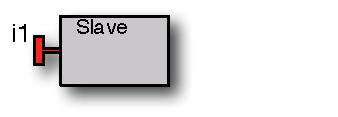
\includegraphics[scale=1]{figures/chapter5/starter.pdf}
		\caption{\textit{starter} application }		
		\label{fig:painlessstarter}

	\end{minipage}
	\hspace{0.25cm}
	\begin{minipage}[b]{0.65\linewidth} 
	\centering
 
		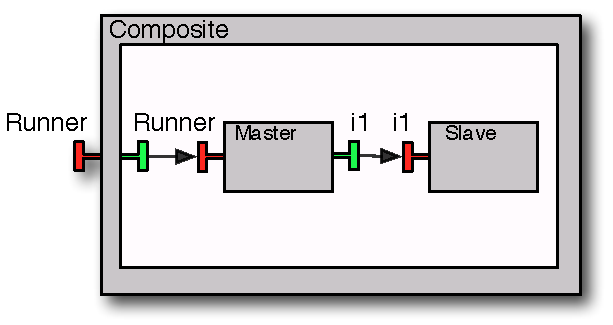
\includegraphics[scale=0.5]{figures/chapter5/composite.pdf}
		\caption{\textit{composite} application }		
		\label{fig:painlesscomposite}
 
	\end{minipage}
	\end{figure}	  		


	\noindent The \textit{starter} application is simply a primitive component named \textit{Slave},
	containing an external, server interface named \textit{i1}. Listing \ref{lst:helloworld} exemplifies one way to define  
	its architecture in \textsc{Painless}.


	\lstinputlisting[language=Painless, stepnumber=1, caption=A first \textsc{Painless} specification, label=lst:helloworld]{listings/chapter5/painlesshelloworld.tex}
	
	
	\noindent We use the previously defined function \textsf{itf}, which belongs to \textsc{Painless} 
	standard library along with other facilities for coping with common operations.
	
	The \textit{starter} application is rather 	simple and acts as an appetizer. % on how to architect GCM/ProActive applications.
	The subsequent \textit{composite} tutorial is slightly more elaborated. Its specification
	is depicted by Listing \ref{lst:composite}. All the involved functions are part of the standard library.
	
		\lstinputlisting[language=Painless, stepnumber=1, caption=\textsc{Painless} specification for the \textit{composite} tutorial, label=lst:composite]{listings/chapter5/painlesscomposite.tex}

	\noindent Firstly, we require the \textit{starter} ADL as defined in Listing \ref{lst:helloworld} (line 1). This, 
	imports all its declarations, namely \textsf{i1} and \textsf{slave}. We proceed by declaring the involved elements (lines 4-11),
	where the only doubt may arise from the \textit{clientof : interface $\rightarrow$ interface} 
	function (line 7). This function returns a \textsf{client} version of the \textsf{interface} given as argument. Finally,
	we deploy the application by making the \textit{composite} component and its two bindings (lines 13-15). The function \textit{add\_subcomponents : component $\rightarrow$ list component $\rightarrow$ component} 
	adds the \textit{master} and \textit{slave} components to the \textit{composite} one,	
	while taking into account all the intricacies regarding their \textit{path}s.		
				
	
	%The equivalent description using the GCM ADL is omitted for the sake of space.

	The last remaining ingredient concerns architectural reconfigurations. %In \textsc{Painless}, these are
	%also included in the ADL, therefore revealing a much more complete picture of the application. For instance,
	Concerning the \textit{composite} example, one could want to replace the \textit{slave} component
	by another one with a different implementation. This can be achieved by appending the reconfiguration
	depicted by Listing \ref{lst:reconfig}, where \textit{mk\_in : path $\rightarrow$ component $\rightarrow$ component} 
	makes the given \textsf{component} in the specified path, and 
	\textit{change\_class : string $\rightarrow$  component $\rightarrow$  component} returns the given \textsf{component}
	with a modified \textsf{class} field.
	

	\lstinputlisting[language=Painless, stepnumber=1, firstnumber=16, caption=\textsc{Painless} reconfigurations, label=lst:reconfig]{listings/chapter5/reconfigs.tex}

	\noindent Basically, we need to unbind the \textit{slave} component before removing it (lines 18-19), 
	make a new \textit{slave}, inside the \textit{composite}, with a different implementation class (line 20),
	and finally bind this new \textit{slave} (line 21). %This reconfiguration is valid as we perform
	%the operations in an adequate order. An invalid reconfiguration is rejected and yields 
	%an exception containing its cause.
	
		
	
	%Last, it should be seen that from a programming perspective, applying this reconfiguration is achieved by a simple method call,
	%while all the machinery involving \textsf{well formed} and \textsf{well typed} concerns
	%occurs in a transparent manner.

%\subsection{Integration with ProActive}
%\label{sub:pro}	
	
	
%	\lstinputlisting[language=Java, stepnumber=1, caption=\textsc{Painless} ProActive application deployment and reconfiguration, label=lst:javacode]{listings/painlessmain.tex}



%\subsection{\textsc{Painless} Reconfiguration}
%\label{sub:preconfig}	

%runtime stuff goes here? 


%a new ADL	
%detail integration with ProActive	
%compare use of PainlessFactory
%functions that carry back origin of error
%ocaml-java
%\cite{conf/sfp/Clerc12}
	
%compare old XML adl with new painless ADL
%code changes are minimal: show them

%eases deployment : real customers have different setups

%hypermanager
%model generation for MC is now fully specified.
%new info can be used to constraint model

%\begin{figure}%[H]
%		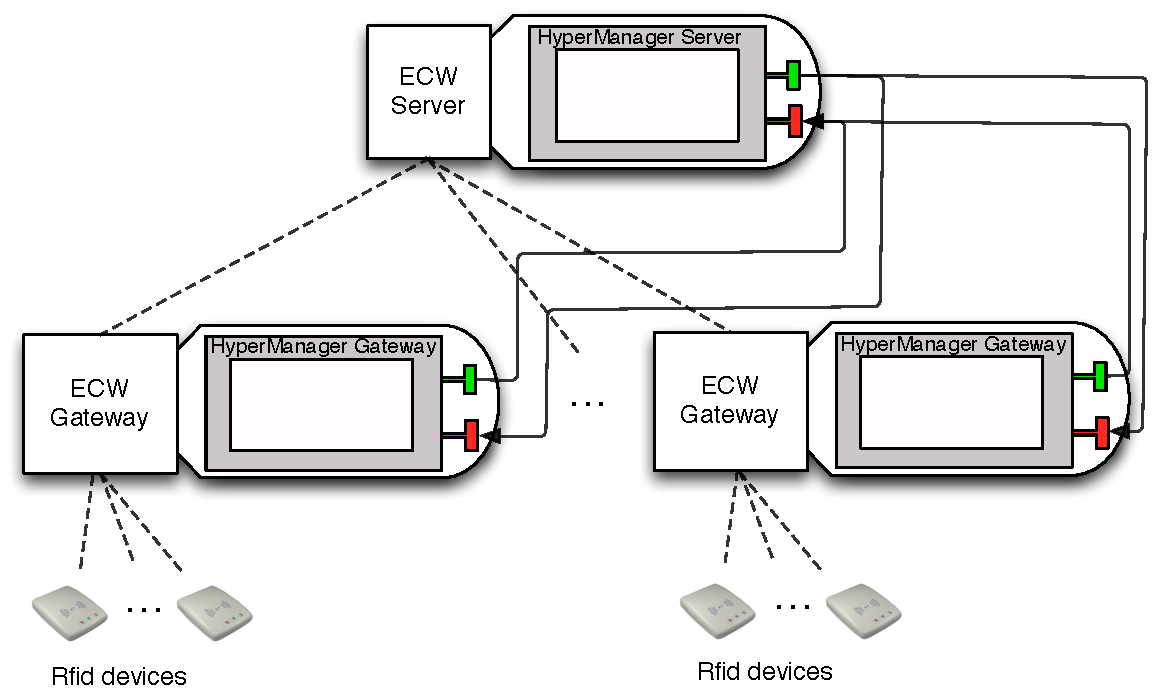
\includegraphics[scale=0.42]{img/architecture.pdf}
%		\caption{Hierarchical representation of the HyperManager case study}		
%		\label{fig:hierarchy}
%	\end{figure}




\section{Discussion}
\label{sec:painlessdiscussion}



In this Chapter we presented \textsc{Painless} and its related novel approach for the
 specification of software architectures. Its declarative trait allows for intuitive
 and concise specifications, liberating the software architect from 
 highly verbose specifications such as the ones obtained via 
 machine languages like XML. Moreover, its support for parametrized 
 architectures eases deployment --- it becomes a 
 matter of instantiation ---, and thus boosts productivity. Further,
 in GCM/ProActive, mapping components to physical resources 
 is achieved through \textit{application/deployment descriptors}. 
 While this information is not an aspect
 of the architecture \textit{per se}, extending \textsc{Painless}
 with such feature could be envisaged.
 
 
 	Another key ingredient is the treatment
 of structural reconfigurations as first-class citizens. Indeed, by supporting
 the specification of the topological changes that may occur at runtime,
 it yields a better understanding of the application. Moreover, it is worth noticing
 that the specified reconfigurations become easily accessible from a programming 
 perspective: through a simple method call with the name of the desired reconfiguration.
 Furthermore, reconfiguration specifications are evaluated	 at runtime.
 The clear benefit is that one can be highly confident that the reconfiguration will
 not let the application in a ill-formed or ill-typed state as
 the evaluation process is carried out by provably correct code extracted from
 \textsc{Mefresa}.
 
 Additionally,  a further inherent advantage is that it all happens without 
 stopping the application. Indeed, actually performing the
 reconfiguration requires it to be stopped at the composite level.
 By making a prior evaluation, the risk of reconfiguration 
 failure is diluted. 
 

 %	The acceptance of a new piece of software can be arduous. Indeed, people
% 	are creatures of habits. With this in mind, all the machinery around \textsc{Painless} 
% 	was designed so that little burden comes from its use. Indeed, adapting a previous GCM/ProActive
%	code for \textsc{Painless} is usuall`y achieved by a one-line adjustment: one should
%	use the \textit{PainlessFactory} to instantiate the application.
  
  
	Composing architecture specifications through the \textsf{Require}
	command fosters reuse, and further contributes to the conciseness
	of \textsc{Painless} specifications. Yet, it is fair to say that
	additional experimentation remains to be done in order to fully
	assess the scalability of the approach. 
	  
  
	At last, an interesting direction for future work concerns ensuring provably safe
	reconfigurations, statically. While runtime checks are useful, one may
	desire stronger guarantees statically. This could be achieved by
	identifying useful classes of architectures that would feature
	provably safe reconfiguration operations. This could be achieved
	by leveraging \textsc{Mefresa}'s apparatus so that all specified reconfigurations provably
	yield well-formed and well-typed states, for all 
	possible execution traces.





\chapbreak

	In this Chapter we presented \textsc{Painless}, a new \ac{ADL} supporting parametrized specifications,
	architectural reconfigurations, and with a declarative trait. Further, we discussed its integration with
	the ProActive middleware.
		
		In the following Chapter we describe the mechanization of a behavioural semantics with the
		Coq proof assistant.
	
	
	
	
	
